\section{TERCERA SECCIÓN}

\lipsum[10]
	
	\subsection{Predimensionamiento}

A continuación, se muestra la \autoref{Ca3_Tabla1} con los parámetros necesarios para definir el modelo bilineal de la interfaz de aislamiento.
\begin{table}[!ht]
\centering
\vspace{1.5 mm}
\caption[Parámetros de la interfaz de aislamiento]{\centering\footnotesize Parámetros de la interfaz de aislamiento}
\vspace{1 mm}
\begin{tabular}{|l|c|c|c|}
\hline
\multicolumn{1}{|c|}{Parámetro}     & Símbolo     & Valor  & Unidad            \\ \hline
Rigidez   postfluencia normalizada  & $K_{p}^{*}$ & 36.84  & $1/s^{2}$ \\ \hline
Rigidez   elástica normalizada      & $K_{e}^{*}$ & 368.40 & $1/s^{2}$ \\ \hline
Fuerza   característica normalizada & $Q^{*}$     & 0.133   & $g$               \\ \hline
\end{tabular}
\label{Ca3_Tabla1}
\end{table}


	\subsection{Resultados} \label{subsection:Resul}

\lipsum[11]

Luego de usar los parámetros de la \autoref{Ca3_Tabla1} se obtuvieron los resultados que se muestran a continuación.
	
		\begin{figure}[!h]
	\centering
		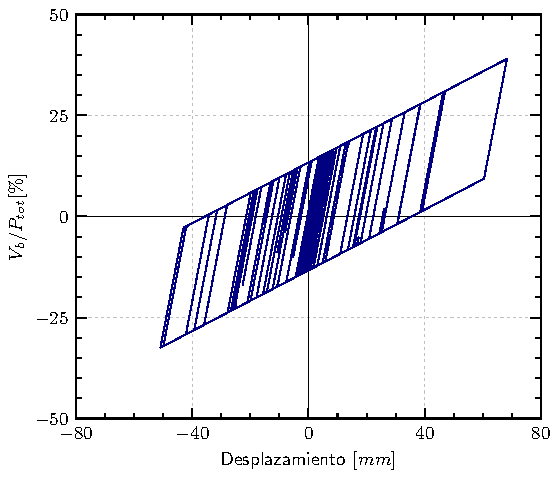
\includegraphics[scale=1]{E_IMAGENES/1_Capitulo3/Cap3_Imagen4.pdf}
		\vspace{-3 mm}
	\caption[Histéresis de la interfaz de aislamiento]{\centering\footnotesize Histéresis de la interfaz de aislamiento.}
	\label{Cap3_Figura4}
	\end{figure}
	

		\begin{figure}[!h]
	\centering
		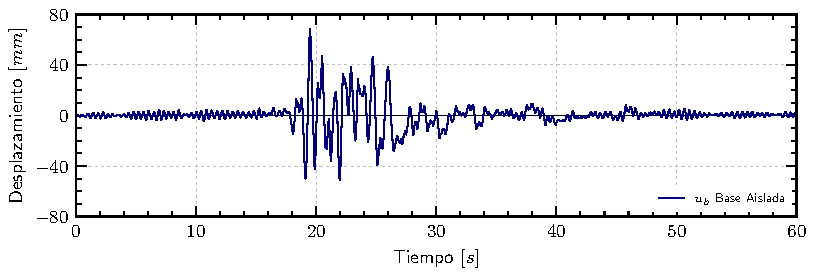
\includegraphics[scale=1]{E_IMAGENES/1_Capitulo3/Cap3_Imagen5.pdf}
		\vspace{-3 mm}
	\caption[Desplazamiento de la interfaz de aislamiento]{\centering\footnotesize Desplazamiento de la interfaz de aislamiento.}
	\label{Cap3_Figura5}
	\end{figure}
		
